\chapter{Introduction to Differential Equations}\label{diffeq}

In this course, we got really good at two things: finding antiderivatives and using power series.  It is no accident that the study of differential equations relies primarily on those two techniques!  Here we show just two methods for solving differential equations: separation of variables, based on antidifferentiation, and power series solutions, based on power series (really!). 

\section{What is a Differential Equation?}

\begin{definition}{Differential Equation}
A \emph{differential equation} (DE) is an equation involving a variable (say $y$) that stands for some unknown function, and also involving one or more derivatives of $y$.  The \emph{solution} to a differential equation is the set of all functions $y$ that make the equation true.
\end{definition}

We begin with a nice bridge troll riddle.  We ask ``What functions are equal to their own derivative?''.

\begin{example}{Functions Equal to Their Own Derivative}

To state this question in the language of differential equations, we say that we wish to solve the DE $$y'=y. $$

\end{example}

\begin{exercise}{Guess and Check \Coffeecup}
Can you think of any functions that are equal to their own derivative?  Do you think you have all of them, or are some likely still out there?
\vspace*{1in}
\end{exercise}
As you can see, guess and check is not a good method for solving even the simplest of differential equations.  We now take a more structured approach.

\section{Separable Equations}

\begin{definition}{Separable}
Let $x$ be the independent variable and let $y$ represent an unknown function of $x$.  A \separable{differential equation} is \emph{separable} if and only if it can be written in the form $$ \frac{dy}{dx}=F(x)G(y)$$ for some functions $F$ and $G$. 
\end{definition} 

Our method for \integ{solving a separable differential equation} is as follows:

\begin{enumerate}
\item Write right-hand side of the differential equation in factored form, one function of $x$ times one function of $y$. 
\item Separate variables by multiplying both sides by $\frac{1}{G(y)}\dif x$.
\item Antidifferentiate both sides.   
\item Solve for $y$, if possible.  (If not, we at least have an implicit solution.)
\end{enumerate}

We try out this method on the previous example.

\begin{example}{Separation of Variables}
Notice the differential equation $$y'=y $$ is \diffeq{separable} because it can be rewritten as  $$\frac{\dif y}{\dif x}=(1)(y). $$
That is, our factored form uses the functions $F(x)=1$ and $G(y)=y$.  We now perform \antider{separation of variables} and antidifferentiate both sides.
\begin{align*}
\frac{1}{y}\dif y &= 1 \dif x \\
\int \frac{1}{y}\dif y &=\int 1 \dif x \\
\ln|y|&=x+C \\
|y|&=e^{x+C} \\
y&=\pm e^{C}e^x \\
y&=Ce^x \\
\end{align*}
Notice that on the last line for simplicity, we clean up the constant $\pm e^C$ by just calling it $C$.
\end{example}

\begin{exercise}{Analyzing the Example \Coffeecup}
\begin{itemize}
\item Why were we able to just put a $+C$ on one side when we integrated?  What would have happened if we put it on both sides? \vspace*{.5in}
\item When we renamed $\pm e^C$ as $C$, we technically introduced a new solution.  The expression $\pm e^C$ is incapable of being equal to zero, but $C$ can be.  Verify that the $C=0$ solution is valid to include as a solution to the differential equation.
 \vspace*{.5in}
\end{itemize}
\end{exercise}

\begin{exercise}{More Complicated DEs \Coffeecup \Coffeecup \Coffeecup}

\begin{itemize}
\item Solve the following differential equation via separation of variables: $$ \frac{dy}{dx}=xy+x $$
\vspace*{2in}
\item  Solve the following Initial Value Problem  via separation of variables: $$ \frac{dy}{dx}=e^{y-x}\sec(y)(1+x^2) $$ Note that you will not be able to obtain an explicit formula for $y$ in terms of $x$ but rather an implicit solution.  Use the initial condition $ y(0)=0$ to solve for $C$.
\vspace*{4in}
\end{itemize}
\AnswerKeyEntry{Any solution to $\frac{dy}{dx}=xy+x$ can be written as $y=Ce^{\frac{x^2}{2}}-1$ for some real number $C$.  The second DE with initial condition has the solution $$\frac{1}{2}e^{-y}\left(\sin(y)-\cos(y)\right)=-e^{-x}\left(3+2x+x^2\right)+\frac{5}{2}. $$}
\end{exercise}

\section{Power Series Solutions} Power series provide a very effective method for solving \series{\powerseries{differential equations}}.  The steps are simple:
\begin{itemize}
\item Set the unknown function $y$ equal to an unknown power series.
\item Plug the power series in for all occurrences of $y$.  Expand and combine like terms. 
\item Equate coefficients one degree at a time (much like we do when solving for unknowns in a PFD).
\item Solve for the coefficients $a_0$, $a_1$, $a_2, \ldots$ one at a time in terms of $a_0$. 
\item Plug those coefficients back into the power series expansion for $y$ to obtain a \diffeq{power series solution}. \item Try to recognize that power series as a known function or variant thereof.  
\end{itemize}
The process is thus very mechanical, but sometimes working through the details becomes a bit messy.  We repeat the previous example with this new method.

\begin{example}{Revisiting Our First DE}
Here we solve $$y'=y $$ using power series.  First, let $y$ be written as a generic unknown power series as follows: $$y(x)=a_0+a_1x+a_2x^2+a_3x^3+a_4x^4+\cdots $$ Plug this expression into the differential equation and expand. \begin{align*}\left(a_0+a_1x+a_2x^2+a_3x^3+a_4x^4+\cdots \right)'&=a_0+a_1x+a_2x^2+a_3x^3+a_4x^4+\cdots \\
a_1+2a_2x+3a_3x^2+4a_4x^3+\cdots &=a_0+a_1x+a_2x^2+a_3x^3+a_4x^4+\cdots \\
\end{align*}
We now equate coefficients one degree at a time, and solve for every coefficient in terms of $a_0$.
\begin{center}
\begin{tabular}{lrcl}
Degree 0: & $a_1=a_0$ & $\implies$ & $a_1=a_0$ \\
Degree 1: & $2a_2=a_1$ & $\implies$ & $a_2=\frac{1}{2}a_0$ \\
Degree 2: & $3a_3=a_2$ & $\implies $& $a_3=\frac{1}{3!}a_0$ \\
Degree 3: & $4a_4=a_3$ & $\implies $& $a_4=\frac{1}{4!}a_0$ \\
\hspace{.2in} \vdots  & \vdots \hspace{.2in} & &\hspace{.17in} \vdots \\
Degree $n-1$: & $na_n=a_{n-1}$ & $\implies$ & $a_n=\frac{1}{n!}a_0$ 
\end{tabular}
\end{center}

We can now plug all coefficients back into our expression for $y$ and simplify until we obtain a closed form for $y$.  \begin{align*}
 y(x)&=a_0+a_0x+\frac{1}{2!}a_0x^2+\frac{1}{3!}a_0x^3+\frac{1}{4!}a_0x^4+\cdots \\
 &=a_0\left(1+x+\frac{1}{2!}x^2+\frac{1}{3!}x^3+\frac{1}{4!}x^4+\cdots \right)
\\
&=a_0e^x
\end{align*}
\end{example}

Notice we have obtained the same solution as via separation of variables!  Clearly, the power series solution was way more work.  The reason it is so valuable though is that there are many DEs which are not separable but for which the power series method works just fine.
\begin{exercise}{Comparing the Methods \Coffeecup \Coffeecup \Coffeecup}
\begin{itemize}
\item \begin{itemize}
\item Show the differential equation $\frac{dy}{dx}=yx$ is separable and use this to separate variables and solve the differential equation.

\vspace*{2in}

\item Solve the same differential equation via power series. Confirm you get the same answer.

\vspace*{2in}

\end{itemize}

\item \begin{itemize} \item Explain why the differential equation $\frac{dy}{dx}=yx+x+1$ is not separable.

\vspace*{1in}

\item Solve the same differential equation via power series.

\vspace*{4in}

\item Check your answer is correct by plugging it back into the original DE.

\vspace*{1in}

\end{itemize}

\item Consider the DE given by $$ y(0)=1 $$ 
$$y'(0)=0 $$
$$ y''=-y.$$

Solve this DE via power series (use the initial conditions to solve for $a_0$ and $a_1$).

\vspace*{4in}

\end{itemize}
\end{exercise}

\section{Modeling with Differential Equations}  Differential equations are used extensively in applied mathematics and the sciences to describe models, which are then solved using mathematics to find explicit formulas for the quantities of interest.

\begin{example}{Newton's Law of Cooling}
Newton's Law of Cooling states that the rate of change of the temperature of a small object in a room is proportional to the difference between room temperature and the temperature of the object.  If $A$ is the constant that represents the ambient temperature (room temperature), $T(t)$ represents the temperature of the room at time $t$, and $k$ is the constant of proportionality, then this situation can be modeled by $$ \frac{dT}{dt}=k(T-A).$$

Here we introduce the idea of a \emph{slope field}, a grid of small dashes that indicate the slope $\frac{\dif T}{\dif t}$ at every point $(t,T)$ in the plane.  Here we draw a slope field that governs solution curves to this model and show one sample solution curve.

\begin{center}
	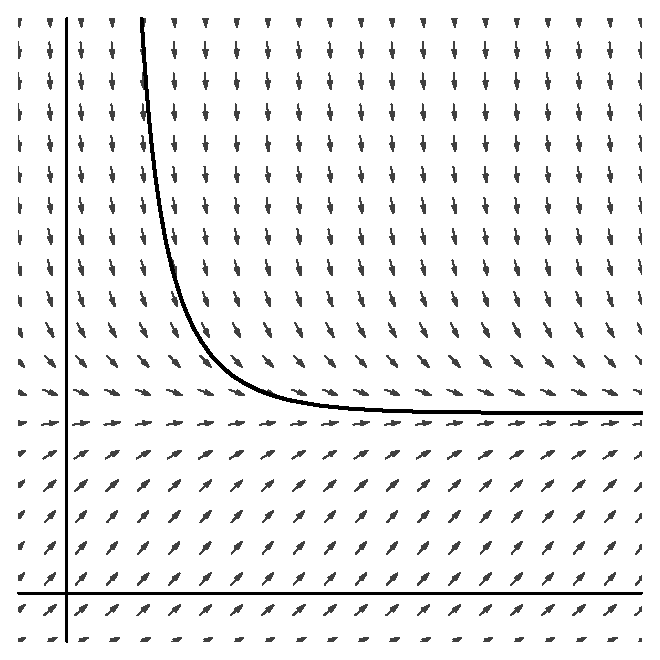
\includegraphics[width=300pt]{ChapterDiffEq/Figures/slopeyfield.eps}
\end{center}

\end{example}

\begin{exercise}{Newton's Law of Cooling \Coffeecup \Coffeecup }
\begin{itemize}
\item Label the above diagram.  What variables do the axes correspond to?  Can you find where the horizontal line $T=A$ is located?
\vspace*{.5in}
\item  In this model, would it make sense that the proportionality constant $k$ is positive or negative?  Why?
\vspace*{.5in}
\item Solve the differential equation by separation of variables. 
\vspace*{2in}
\item Solve the differential equation by power series. 
\vspace*{4in}
\end{itemize}
\end{exercise}
Note that those solutions give explicit formulas for the solution curves above, which is significantly more useful than just thinking of it intuitively as ``following the arrows''.

\begin{exercise}{ Malthusian Population Model }

A simple intuitive population model can be stated as follows:

\begin{center}
\emph{If there are more individuals in a population, there will be more babies produced.}
\end{center}

Here is a slightly more technical restatement of the same idea:

\begin{center}
\emph{The rate of growth of a population is proportional to the size of the population.}
\end{center}

\begin{itemize}
\item Let $P(t)$ be the size of the population at time $t$.  Rewrite the above growth principal in the language of differential equations.
\vspace*{1in}
\item Solve your differential equation using power series. 
\vspace*{5in}
\item Solve your differential equation using separation of variables and confirm that your answers match.
\vspace*{2in}
\item Use your formula to find the limit of $P(t)$ as $t$ approaches infinity.  
\vspace*{2in}
\item Under what real life conditions might this model be realistic?  Under what conditions might this model be unrealistic?
\vspace*{2in}
\end{itemize}
\end{exercise}

As you probably noticed, the above model is slightly ridiculous for large time values since it would claim that eventually any species would fill up the entire visible universe with bodies.  So let's adjust it to fix that unrealistic assumption. Here's an upgrade:

\begin{exercise}{ Logistic Population Model \Coffeecup \Coffeecup \Coffeecup}

\begin{center}
\emph{If there are more individuals in a population, there will be more babies produced, but then it slows down as it approaches some sort of maximum possible population (a limit perhaps based on food supply, available habitat, etc).}
\end{center}

Here is a slightly more technical restatement of the same idea:

\begin{center}
\emph{The rate of growth of a population is jointly proportional to both the size of the population and the distance from some maximum possible population.}
\end{center}

\begin{itemize}
\item Let $P(t)$ be the size of the population at time $t$ and let $M$ for maximum be a constant that the population cannot exceed.  Rewrite the above growth principal in the language of differential equations.
\vspace*{1in}
\item Solve your differential equation using power series out to a degree two approximation (this will be much too difficult to solve the whole thing using power series!). 
\vspace*{4in}
\item Solve your differential equation using separation of variables and confirm that your answers match out to the degree two approximation.
\vspace*{2in}
\item Use your formula to find the limit of $P(t)$ as $t$ approaches infinity.  
\vspace*{2in}
\item Suppose you started with population $P(0)=2M$.  What would your model predict would happen to the population?
\vspace*{2in}
\end{itemize}
\end{exercise}
